\begin{figure*}[t]
\centering
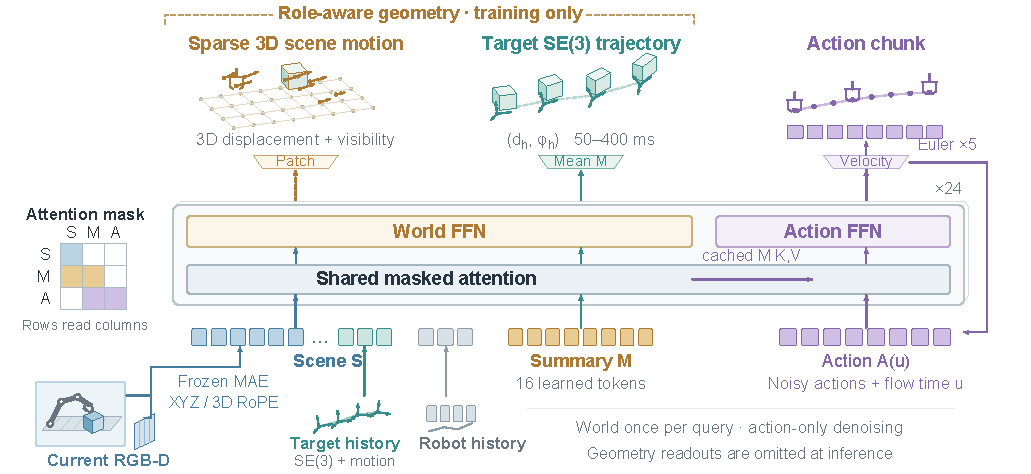
\includegraphics[width=\textwidth]{figures/Fig2/fig2_se3wam.pdf}
\caption{\textbf{\ours architecture.}
(a) Current RGB-D and target/robot histories form scene tokens $S$, alongside learned summaries $M$ and noisy actions $A$.
Each layer shares masked attention, applies one World FFN to $S,M$ and a separate Action FFN to $A$, and retains both residual updates.
Final patch and mean-summary states support training-only geometric readouts (dashed); actions read hidden states.
(b) Mask rows are queries and columns are keys.
(c) Joint training combines auxiliary supervision and action flow matching. At deployment, world prefill caches layer-wise keys and values for action sampling, skipping geometric readouts.
The RGB thumbnail is a Blender rendering. Geometric examples show recorded supervision (flow enlarged); token counts, layer stacking and action icons are schematic.}
\label{fig:architecture}
\end{figure*}
